\documentclass{beamer}
\usetheme{Copenhagen}
\definecolor{kured}{RGB}{77,137,99}
\definecolor{titlegreen}{RGB}{77,137,99}
\usecolortheme[named=kured]{structure}
\usepackage[sort]{natbib}
\usepackage[tight]{subfigure}
% Components of the title page
\title[Predicción del precio del Bitcoin.]{Predicción del precio del Bitcoin mediante ventanas móviles y un ensamble de estimadores por Modelos Lineales modelados a través de Bagging con Árboles de Regresión.}
\subtitle{}
\author[Vanessa A., Pablo M. A.]{Vanessa Alcalde, Pablo Martinez Angerosa}
\institute[IESTA]{ Análisis Multivariado II}
\date[L24H :: 17-12-2020]{Diciembre 17, 2020}

%
\begin{document}

% Frame 1
\frame[plain]{\titlepage}



% Frame 2
\begin{frame}[t]
\frametitle{Introducción}


\vfill

\begin{itemize}

\item Bitcoin, una criptomoneda digital esta actualmente siendo integrada y aceptada por los principales actores del mundo de las finanzas.
\item Existen diversas investigaciones que analizan la composición del precio del Bitcoin.
\item Bitcoin es un paseo aleatorio.
\item El algoritmo recomendado para la predicción del precio del Bitcoin es Modelos Lineales.
\item Variables explicativas recomendadas están compuestas de rezagos del precio y el volumen del Bitcoin. 

\end{itemize}


\vfill
\end{frame}

% Frame 3
\begin{frame}[t]
\frametitle{ Introducción}
\center
\vfill
\begin{itemize}

\item Objetivo proponer alternativas a las investigaciones realizadas actualmente que mejoren el rendimiento. 
\item Se utilizó un sistema de ventanas móviles el cual genera un ensamble de estimadores mediante Modelos Lineales, que son consideradas como opiniones expertas, y se proponen diversas técnicas para sintetizar estas opiniones en una sola predicción.
\item El modelo propuesto logra duplicar el rendimiento de otras técnicas.
\end{itemize}
\vfill
\end{frame}

% Frame 4
\begin{frame}[t]
\frametitle{ Datos - Descripción de los datos}
\center
\vfill
\begin{itemize}
\item 
Se utilizan los datos por hora del precio de $Cierre$ y $Volumen$ de transacciones de Bitcoin.
\item Los datos se descargan de la API de Binance.
\item Registros históricos por hora en dólares americanos (USD) de Bitcoin(BTC). 
\item La base de datos contiene 8717 registros comenzando en el día $12/12/2019$ a las 08:00:00h hasta el $10/12/2020$ a la 01:00:00h.
\vfill
\end{itemize}

\end{frame}

% Frame 5

\begin{frame}[t]
\frametitle{ Datos - Preparación de los datos}

\vfill
\centering
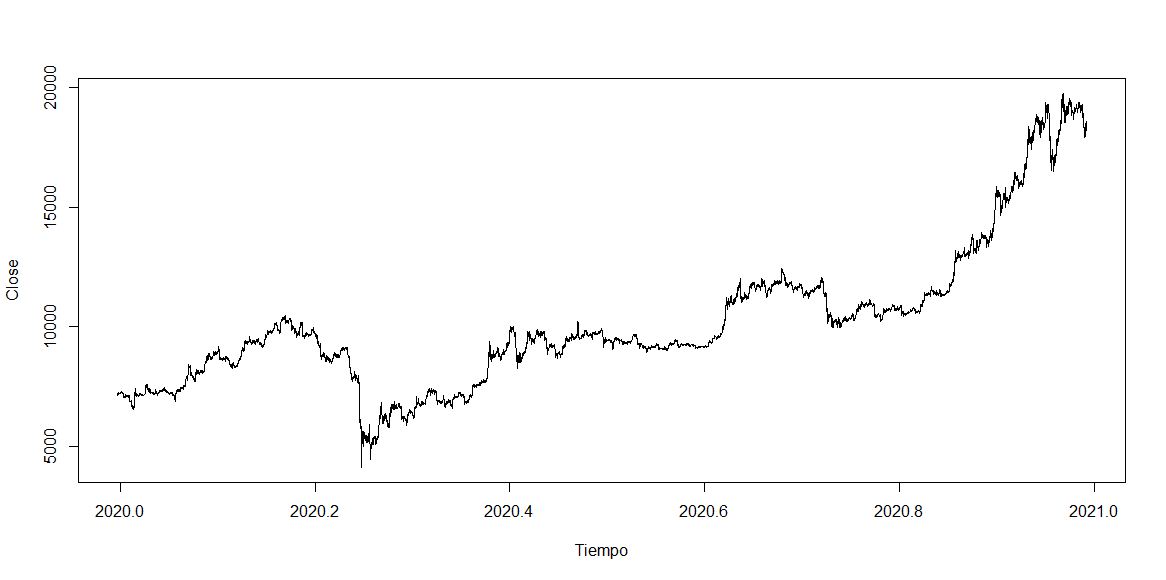
\includegraphics[width=1\textwidth]{serie}
Serie de Tiempo del precio del $Cierre$ por hora del Bitcoin desde el día $12/12/2019$ a las 08:00:00h hasta el $10/12/2020$ a la 01:00:00h.

\end{frame}

% Frame 6
\begin{frame}[t]
\frametitle{ Datos - Preparación de los datos}

\vfill
\begin{itemize}
\item 
La variable de predicción $Y$ corresponde al $Cierre$ del precio del Bitcoin en el tiempo $n$. 
\item 
Se crearon variables de rezagos llamadas $lag$, para el precio de $Cierre$ y $Volumen$ de Bitcoin.
\item 
Cinco primeros rezagos del precio del $Close$ y del $Volumen$ del Bitcoin. 
\item
Variables son definidas como $closeLag1$, $closeLag2$, $closeLag3$, $closeLag4$, $closeLag5$, $volLag1$, $volLag2$, $volLag3$, $volLag4$ y $volLag5$, respectivamente.

\vfill
\end{itemize}

\end{frame}
% Frame 7
\begin{frame}[t]
\frametitle{ Metodología - Modelos Lineales}

\vfill
\begin{itemize}
\item 
Las 4 técnicas utilizadas fueron Modelos Lineales, Métodos de Ensamble de Modelos, Bagging basado en Árboles de Decisión y Redes Neuronales.
\item 
Un modelo de regresión lineal múltiple (\ref{ecuacionML}) es un Modelo Lineal en los parámetros en el cual la variable de respuesta, $Y$, es determinada por un conjunto de variables independientes, las variables explicativas (matriz $X$). Se busca el hiperplano que mejor ajuste a los datos. Los parámetros $\beta_i$ para el modelo se obtienen por mínimos cuadrados.

\begin{equation}
y_{i}=\beta_{0}+\beta_{1} x_{i}+\beta_{2} x_{i}+\cdots+\beta_{d} x_{i}+\epsilon_{i}
\label{ecuacionML}
\end{equation}
\vfill
\end{itemize}

\end{frame}

% Frame 8
\begin{frame}[t]
\frametitle{Metodología - Métodos de Ensamble de Modelos}

\vfill
\begin{itemize}
\item 
Los Métodos de Ensamble de Modelos son útiles para mejorar el rendimiento de los modelos de aprendizaje automático al mejorar su precisión. 
\item 
Se construyen varios modelos y se combinan las predicciones resultantes promediando. 
\item 
Este promedio de errores produce mejores predicciones generalizando el carácter particular de cada uno de estos modelos.


\vfill
\end{itemize}

\end{frame}

% Frame 9
\begin{frame}[t]
\frametitle{Metodología -  Árbol de Decisión }

\vfill
\begin{itemize}
\item 
Un árbol de decisión es una división recursiva del espacio de variables explicativas en una estructura en forma de árbol, cada nodo interior contiene una pregunta sobre una variable de entrada y cada nodo terminal una decisión. 
\item Pueden ser utilizados en problemas de regresión y clasificación. 
\item 
Los árboles CART (Classification And Regression Tree) se construyen dividiendo el conjunto de valores posibles de $X_1,X_2,...,X_p$ en $J$ regiones disjuntas $R_1, R_2,..., R_J$. En el caso de un árbol de regresión, para cada observación en la región $R_j$ se predice el valor medio de las respuestas.

\vfill
\end{itemize}

\end{frame}

% Frame 9
\begin{frame}[t]
\frametitle{ Metodología -  Árbol de Decisión}

\vfill
\begin{itemize}

\item 
Para llevar a cabo la construcción del árbol se comienza con un conjunto de datos de entrenamiento, el cual es segmentado mediante particiones binarias. Se crean regiones $R_1, R_2,..., R_J$ de manera que se minimice la Ecuación (\ref{ecuacionTree}).


\begin{equation}
\sum_{j=1}^{J} \sum_{i \in R_{j}}\left(y_{i}-\hat{y}_{R_{j}}\right)^{2}
\label{ecuacionTree}
\end{equation}


Donde $\hat{y}_{R_{j}}$ es la respuesta media para las observaciones del conjunto de entrenamiento en la región j-ésima.
\item
Una vez que se encuentra la mejor partición, se separan los datos en las regiones resultantes y se repite el proceso. Este proceso termina cuando se satisface algún criterio de parada.
\vfill
\end{itemize}

\end{frame}


% Frame 10
\begin{frame}[t]
\frametitle{Metodología - Bagging (Bootstrap Aggregating)}

\vfill
\begin{itemize}
\item 
Método para reducir la varianza de un modelo de aprendizaje automático.
\item 
Se divide el conjunto de datos en entrenamiento $L$ y testeo $T$, se toma una muestra bootstrap $L_b$ de $L$ y se construye un estimador usando $L_b$. Se repite el procedimiento $B$ veces. Luego a cada dato de $T$ se le asigna el promedio de las respuestas de los estimadores construidos en el paso anterior (para el caso de un modelo de regresión). La proporción de veces que la clase estimada difiere de la verdadera es el error Bagging.
\item 
Bagging para Árboles de Decisión: se construyen $B$ árboles con conjunto de entrenamiento obtenido mediante una muestra bootstrap del conjunto de entrenamiento original, luego se hace un promedio de las predicciones resultantes. Esto reduce la varianza, lo que mejora la precisión de las predicciones.
\vfill
\end{itemize}

\end{frame}

% Frame 11
\begin{frame}[t]
\frametitle{ Metodología - Redes Neuronales }
\vfill
\begin{itemize}
\item 
Las Redes Neuronales son un modelado matemático que homologa el comportamiento de una neurona biológica. El objetivo de su diseño es emular al cerebro humano.   
\item
Se construyen combinaciones lineales de las entradas y se obtiene la salida como una función no lineal de estas. 
\end{itemize}
\centering
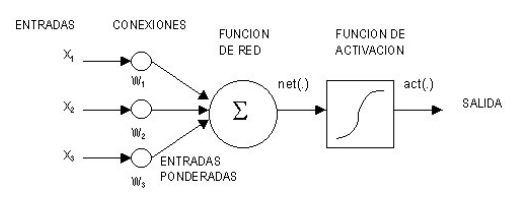
\includegraphics[width=0.65\textwidth]{redNeuronal}
\vfill
\end{frame}

% Frame 11
\begin{frame}[t]
\frametitle{ Metodología - Redes Neuronales }
\vfill

Se muestra el modelado de una red neuronal con una capa de entrada, una capa oculta y una salida. Donde $i$, $j$ son los índices correspondientes a la capa de entrada y oculta respectivamente, $w$ corresponde a los pesos de cada neurona y $f(.)$ a la función de activación.

\begin{block}{}
\centering
$g_{k}(x)=f \underbrace{(\sum_{j=1}^{n_{H}} w_{k j} f \underbrace{\left(\sum_{i=1}^{d} w_{j i} x_{i}+w_{j 0}\right)}_{\text {net }_{j}}+w_{k 0})}_{\text {net }_{k}}$
\end{block}
\vfill
\end{frame}

% Frame 11
\begin{frame}[t]
\frametitle{ Metodología - Redes Neuronales }
\vfill
\begin{itemize}
\item
El procedimiento para encontrar los pesos que configuren el mejor modelo consiste en primero multiplicar cada dato de entrada por un peso y los valores ponderados se combinan linealmente. 
\item
Posteriormente se aplica una función de activación no lineal. El valor de salida es comparado con el valor objetivo. La diferencia de error que se produce es utilizada para actualizar los pesos y se itera hasta obtener el criterio deseado de parada. 
\item
Actualmente el algoritmo más utilizado para esto es el de Backpropagation. 
\end{itemize}
\vfill
\end{frame}

% Frame 12
\begin{frame}[t]
\frametitle{ Metodología - RMSE}
\vfill

Para evaluar el rendimiento de los distintos modelos de predicción se utilizó la medida de error RMSE.

\begin{block}{RMSE}
$(min)RMSE=\sqrt{\frac{1}{N} \sum_{i=1}^{N}\left(y_{i}-f_{i}\right)^{2}}$
\end{block}

Siendo $y_i$ las predicciones y $f_i$ los valores reales. 
\vfill
\end{frame}

% Frame 12
\begin{frame}[t]
\frametitle{Proceso}

\vfill
\begin{enumerate}
\item 
El conjunto de datos se dividió aleatoriamente, en una muestra de entrenamiento del $70\%$ y una muestra de testeo del $30\%$.
\item 
Se recrea la predicción del precio del Bitcoin mediante la estrategia de Modelos Lineales propuestas en la literatura. 
\end{enumerate}
\begin{itemize}
\item
Se construyó un algoritmo de fuerza bruta que evalúa secuencialmente una a una todas las posibles combinaciones de las variables seleccionadas.
\item
Se compara el RMSE generado por cada una de estas combinaciones con la muestra de testeo. 
\item 
El modelo seleccionado es aquel con el menor RMSE. 

\item Se cuenta con $1023$ posibles modelos.
\end{itemize}



\vfill
\end{frame}
% Frame 12
\begin{frame}[t]
\frametitle{Proceso}
\vfill
Diagrama del proceso de selección del Modelo Lineal con menor RMSE con respecto a la muestra de testeo a partir de un ensamble de $1023$ posibles modelos generados desde las combinaciones obtenidas.
\vfill
\centering
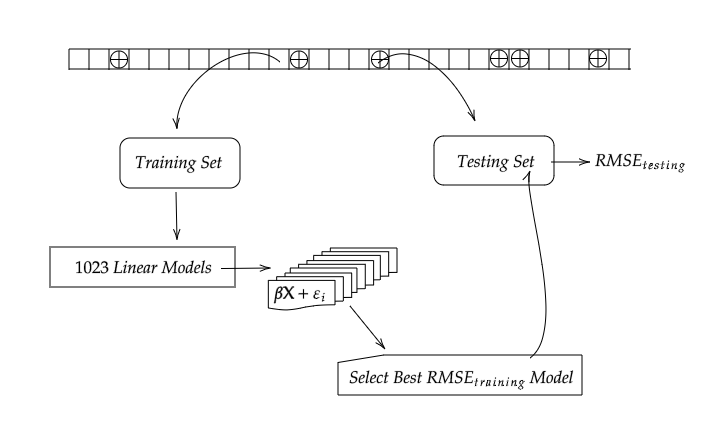
\includegraphics[width=0.75\textwidth]{diagramLinearRegression}
\end{frame}

% Frame 12
\begin{frame}[t]
\frametitle{Proceso - Ventanas móviles}

\vfill
\begin{itemize}
\item
Buscando nuevas alternativas de predicción se introduce el concepto de ventanas móviles.
\item 
Generan un enfoque dinámico de muestras de entrenamiento y testeo.
\item 
Para predecir el precio en el momento $n$ se genera una ventana de $w$ rezagos desde el momento $n-1$ hasta el momento $n-w-1$ (ancho de $w$). 
\item
Se utiliza una ventana móvil de 25 rezagos. 
\item
Para cada momento $n$ que se quiere predecir se genera un ensamble de $1023$ Modelos Lineales, a partir de todas las combinaciones de las variables seleccionadas con una muestra de entrenamiento de ancho $w$.

\vfill
\end{itemize}

\end{frame}
% Frame 12
\begin{frame}[t]
\frametitle{Proceso - Linealidad y precisión del ensamble}
\vfill
\begin{itemize}
\item 
La linealidad en cada una de las ventanas móviles es extremadamente fuerte ya que el RMSE obtenido con las mismas muestras de entrenamiento es considerablemente bajo.
\item 
Utilizar Modelos Lineales sobre el concepto de ventanas móviles es una buena opción.
\item 
Además entre las $1023$ predicciones obtenidas por los modelos lineales en cada ventana en un  $76.15\%$ de los casos al menos uno de los modelos realizaba una estimación casi perfecta en un intervalo $\pm 5$ dólares. 
\vfill
\end{itemize}
\end{frame}

% Frame 12
\begin{frame}[t]
\frametitle{Proceso}
\vfill
Muestra aleatoria de cuatro momentos de la base y las $1023$ predicciones del precio de $Close$.
\vfill
\centering
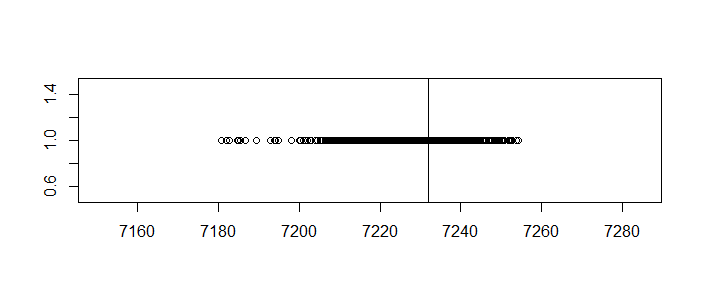
\includegraphics[width=5.0cm]{muestra1}
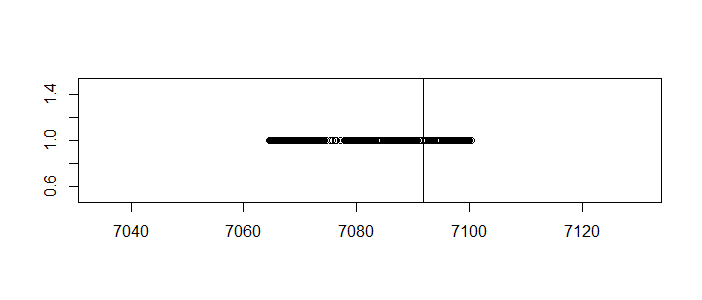
\includegraphics[width=5.0cm]{muestra2}
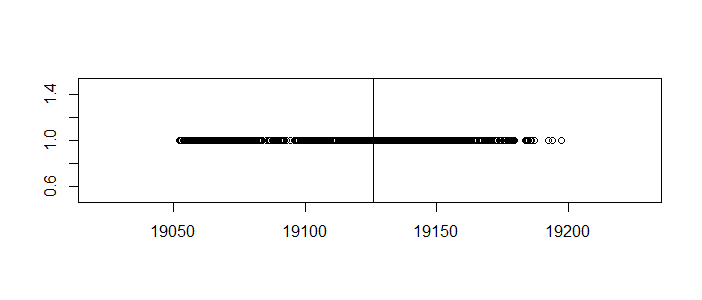
\includegraphics[width=5.0cm]{muestra3}
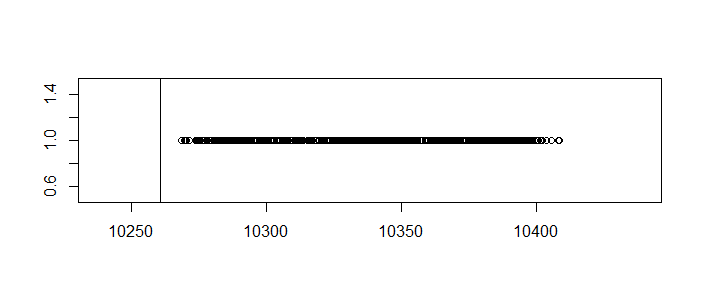
\includegraphics[width=5.0cm]{muestra4}
\end{frame}

% Frame 12
\begin{frame}[t]
\frametitle{Proceso}
\vfill
\begin{itemize}
\item
La estrategia a seguir es  encontrar posibles patrones entre los precios estimados por cada uno de los $1023$ modelos y el precio real de $Close$ del Bitcoin en cada ventana móvil. 
\item
Los posibles patrones a encontrar entre este ensamble de predicciones y el precio real son muchos.
\item
La pregunta fundamental a responder es ¿existe algún patrón entre las $1023$ predicciones por ventana de rezagos y el precio real del Bitcoin?
\item
Se crea una nueva base de datos donde se mantiene la temporalidad de la base anterior pero se cambian las variables explicativas de cada fila. 
\item
Cada una de las filas está compuesta por un ensamble de $1023$ variables que mantienen en orden estricto las predicciones generadas por los $1023$ Modelos Lineales ajustados en la ventana.
\end{itemize}
\vfill
\end{frame}

% Frame 12
\begin{frame}[t]
\frametitle{Proceso}
\vfill
\begin{itemize}
\item
Histograma de frecuencia absoluta de aciertos de los $1023$ modelos en toda la base.
\item
Intervalo de acierto es de $\pm 5$ dólares.
\item
Umbral mínimo que logran todos los modelos es de $351$ ($4.03\%$) aciertos. 
\item
Primer umbral tiene un promedio de acierto de $545.904$ ($6.26\%$).
\item
Segundo umbral tiene un acierto promedio de $713.1167$ ($8.18\%$) 
\item
Tercer umbral tiene un acierto promedio de $887.797$ ($10.19\%$). 
\end{itemize}

\centering
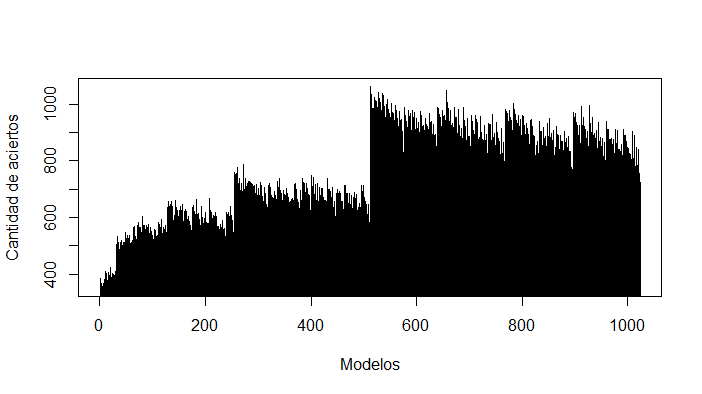
\includegraphics[width=0.5\textwidth]{histograma}

\vfill
\end{frame}

% Frame 12
\begin{frame}[t]
\frametitle{Proceso}
\vfill
\begin{itemize}
\item
Siguientes pasos fueron aplicar algoritmos de aprendizaje automático para buscar la relación entre el ensamble de estimaciones de precios y el precio correcto. 
\item
Utilizamos Métodos de Ensamble de Modelos, Bagging basado en Árboles de Decisión y Redes Neuronales.
\item
Se considera el ensamble de estimaciones ($1023$) por Modelos Lineales como un conjunto de opiniones de expertos.
\end{itemize}
\vfill
\end{frame}

% Frame 12
\begin{frame}[t]
\frametitle{Proceso - Opiniones expertas}
\vfill
Un primer criterio para sintetizar estas opiniones es el algoritmo de Ensamble de Modelos, donde se promedian las opiniones buscando mediar las  más extremas y lograr un consenso. 
\vfill
\centering
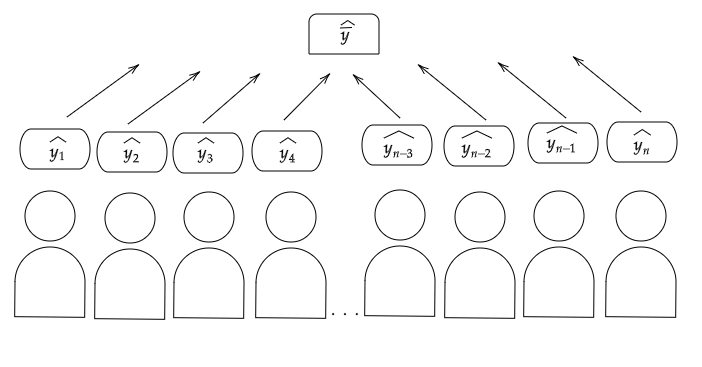
\includegraphics[width=0.65\textwidth]{diagramMeanExpertOpinion}


\end{frame}

% Frame 12
\begin{frame}[t]
\frametitle{Proceso - Ensamble de Modelos}
\vfill
Para cada momento $n$ a predecir de la muestra de testeo se realiza una ventana de $25$ rezagos, se obtienen las $1023$ predicciones para el precio del momento $n$ (opiniones expertas) y se promedian para obtener el precio estimado.
\vfill
\centering
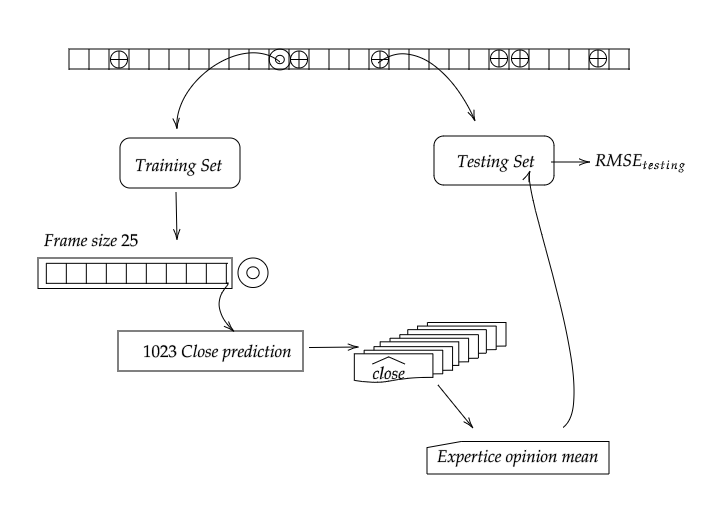
\includegraphics[width=0.75\textwidth]{diagramExpertMean}
\end{frame}

% Frame 12
\begin{frame}[t]
\frametitle{Proceso - Bagging}
\vfill
\begin{itemize}
\item
El segundo criterio fue utilizar Bagging con Árboles de Regresión.
\item
Se ajusta exactamente con la misma muestra de entrenamiento con la que se realizó la primera estimación por Modelos Lineales. 
\item
Con el modelo ajustado, se predice cada una de las muestras de testeo y se calcula el RMSE. 
\end{itemize}
\vfill
\centering
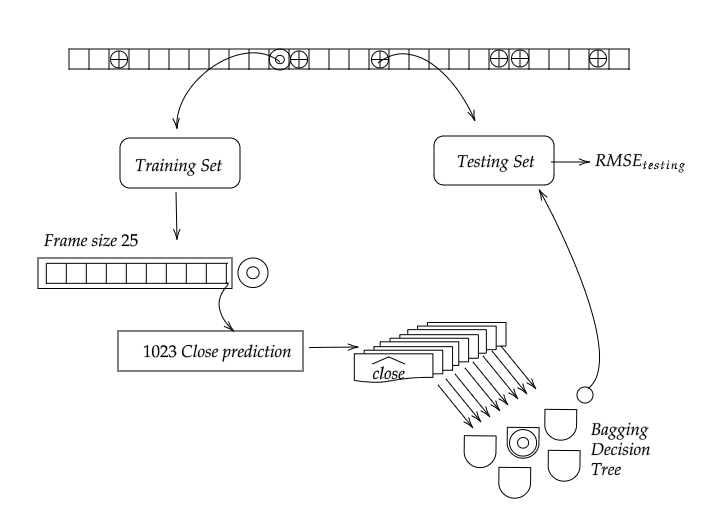
\includegraphics[width=0.5\textwidth]{diagramBagging}
\end{frame}

% Frame 12
\begin{frame}[t]
\frametitle{Proceso - Redes Neuronales}
\vfill
\begin{itemize}
\item
El tercer criterio fue aplicar Redes Neuronales. 
\item
Primero se entrena una red donde sus variables de entrada son el ensamble de $1023$ opiniones de expertos generados por una ventana de $25$ rezagos para cada momento $n$ de la muestra de entrenamiento original.
\item
Se calcula el RMSE con el modelo obtenido sobre la muestra de testeo. 
\end{itemize}
\vfill
\centering
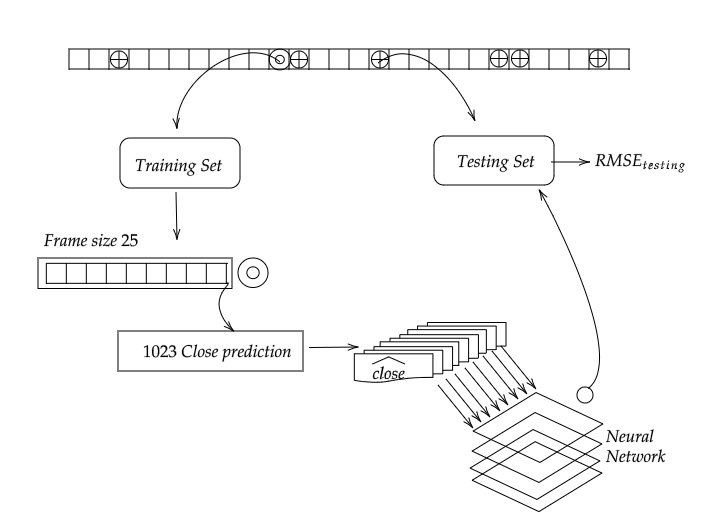
\includegraphics[width=0.5\textwidth]{diagramNeuralNetwork}
\end{frame}

% Frame 12
\begin{frame}[t]
\frametitle{Resultados - Modelos Lineales y Ensamble de Modelos}
\vfill
\begin{itemize}
\item
Objetivo de esta investigación es encontrar metodologías alternativas a investigaciones previas y la literatura y lograr mejorar el rendimiento propuesto. 
\item
El modelo referencia, mediante Regresión Lineal, logra un RMSE de predicción de  $231.45$.
\item
Este modelo está compuesto por dos variables explicativas, $closeLag1$ y $closeLag3$.
\item
El Ensamble de Modelos logra un RMSE de $91.33$ con respecto a las observaciones de la muestra de testeo original. Logra duplicar el rendimiento obtenido por el RMSE de referencia. 
\end{itemize}
\end{frame}


% Frame 12
\begin{frame}[t]
\frametitle{Resultados - Bagging}
\vfill
\begin{itemize}
\item
El algoritmo de Bagging con Árboles de Regresión logra un RMSE resultante de $78.87$ con respecto a las observaciones de testeo de la muestra original. 
\item
Refleja una mayor flexibilidad y complejidad de decisión.
\item
Se utilizaron $100$ árboles y las $1023$ variables de entrada.
\item
Se utilizó el paquete de R randomForest.
\item
Se contrastan las $12$ variables explicativas que tienen más peso en la media de precisión en las predicciones en la muestra cuando cada una se excluye del modelo con el histograma de frecuencia absoluta de aciertos. 
\end{itemize}

\centering
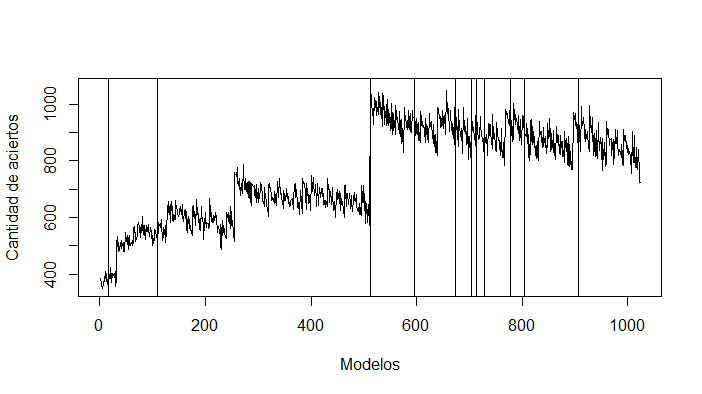
\includegraphics[width=0.5\textwidth]{aciertoBagging}
\vfill
\end{frame}


% Frame 12
\begin{frame}[t]
\frametitle{Resultados - Bagging}
\vfill
\begin{itemize}
\item
En la Figura se muestra como disminuye el error MSE a medida que se aumenta la cantidad de árboles utilizada para Bagging.
\item
Este algoritmo es el que logra el mejor RMSE de todas las propuestas.
\end{itemize}
\centering
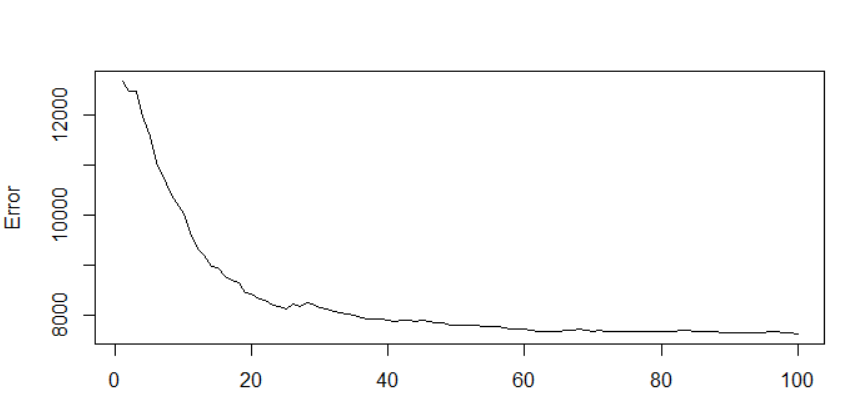
\includegraphics[width=0.5\textwidth]{errorMSEBagging}
\vfill
\end{frame}
% Frame 12
\begin{frame}[t]
\frametitle{Resultados - Redes Neuronales}
\vfill
\begin{itemize}
\item
Se utilizó una Red Neuronal con $1023$ variables de entrada.
Tres capas ocultas.
\item
La primera capa oculta es utilizada para la estandarización de los valores de las variables de entrada.
\item
Las siguientes dos capas están compuestas por 16 y 8 nodos respectivamente.
\item
Una capa de salida.
\item
Todas las funciones de activación son relu.
\item
Se realizó un entrenamiento de $1000$ épocas.
\item
El RMSE con respecto a la muestra original de testeo es de $136.8908$. 
\item
Se utilizó el paquete Keras de R que es una capa de alto nivel de Tensorflow.
\end{itemize}
\vfill
\end{frame}
% Frame 12
\begin{frame}[t]
\frametitle{Resultados - Redes Neuronales}
\vfill
\begin{itemize}
\item
Redes Neuronales es el algoritmo con mayor flexibilidad y complejidad de decisión utilizado.
\item
El rendimiento con menor cantidad de nodos en las capas afecta enormemente de forma negativa el rendimiento de la red.
\item
Este algoritmo obtuvo el peor rendimiento, pero logra superar el rendimiento alcanzado por el modelo de referencia.
\end{itemize}

Este Cuadro muestra las distintas configuraciones de las redes neuronales empleadas y el RMSE.

\begin{table}[!hbt]
\centering
\begingroup\setlength{\fboxsep}{0pt}
\colorbox{lightgray}{%
\begin{tabular}{|l|l|l|l|}
\hline Capa 2 &  Capa 3  &  Activación & RMSE \\
\hline 16 & 8  &  relu &136.89\\
\hline 8 & 8  &  relu &10640.92\\
\hline
\end{tabular}%
}\endgroup
\end{table}
\vfill
\end{frame}
% Frame 12
\begin{frame}[t]
\frametitle{Resultados}
\vfill
\begin{itemize}
\item
En el Cuadro se muestra el desempeño de cada uno de los modelos seleccionados, Ensamble de Modelos, Bagging y Redes Neuronales, comparados con los resultados obtenidos por el modelo de referencia basado en Modelos Lineales. 
\item
Bagging es el que logra mejores resultados. 
\item
Los tres modelos propuestos superan el rendimiento del modelo de referencia original.

\begin{table}[!hbt]
\centering
\begingroup\setlength{\fboxsep}{0pt}
\colorbox{lightgray}{%
\begin{tabular}{|l|l|}
\hline Algoritmo de predicción & RMSE \\
\hline Modelos Lineales & 231.45\\
\hline Ensamble de Modelos & 91.33\\
\hline Bagging (Árbol de Regresión)& 78.87\\
\hline Redes Neuronales & 136.89 \\
\hline
\end{tabular}%
}\endgroup
\end{table}
\vfill
\end{itemize}
\end{frame}

% Frame 12
\begin{frame}[t]
\frametitle{Conclusiones}
\vfill
\begin{itemize}
\item
El objetivo de esta investigación es encontrar técnicas alternativas para la predicción del precio del Bitcoin.
\item
El sistema de ventanas móviles presentado que genera un ensamble de estimadores mediante Modelos Lineales aplicado a la técnica de Bagging obtiene un rendimiento ampliamente mayor que los modelos propuestos originalmente.
\item
Aunque Redes Neuronales no obtuvo los mejores resultados, si mostró una tendencia a la mejora en predicción a medida que se aumentaba la complejidad de las redes. 
\item
El nuevo enfoque presentado en esta investigación aplicado al algoritmo de Bagging sobre Árboles de Regresión se convierte en una opción candidata para la predicción del precio del Bitcoin.
\end{itemize}

\vfill
\end{frame}


% Frame 12
\section*{ }
\begin{frame}[t]
\frametitle{Referencias}
\bibliographystyle{apalike} \bibliography{lswbib}
\begin{itemize}
\item
Gareth, J., Witten, D., Hastie, T., Tibshirani, R. (2013). 
{An introduction to statistical learning: with applications in R.}
New York: Springer.
\item
Alcalde, V., Martinez Angerosa, P. (2020). 
{Predicción del precio del Bitcoin mediante ventanas móviles y un ensamble de estimadores por Modelos Lineales modelados a través de Bagging con Árboles de Regresión.}
\end{itemize}
\end{frame}

\end{document}